\part{Capítulo diez}

%----------------------------------------------------------------------------------------
%	CHAPTER 10
%----------------------------------------------------------------------------------------

\graphicspath{ {10_Capitulo/img/ejemplos/},{10_Capitulo/img/explicacion/}, {W_Varios/2_Portada_capitulos/} }


\chapterimage{ima2} % Chapter heading image

\chapter{Costo anual uniforme equivalente}

\begin{center}
	\textbf{\Large Corrección de nomenclatura, formulación, ejemplos y criterios de decisión}
\end{center}
\vspace{0.3cm}

\section{Mapa mental}
\begin{figure}[h]
	\centering
	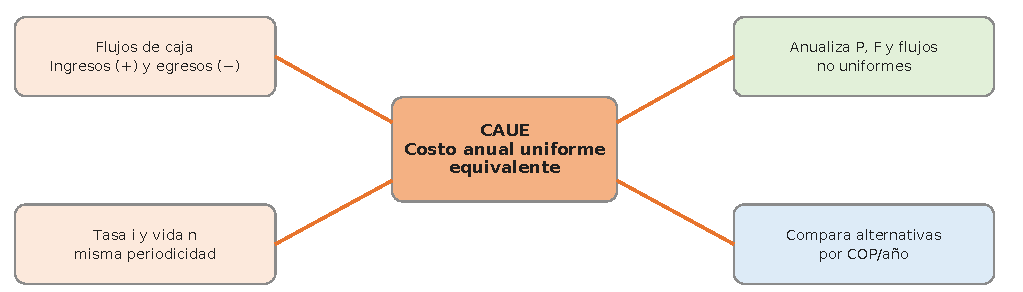
\includegraphics[width=\textwidth]{10_Capitulo/img/explicacion/Mapa Mental 10.1.pdf}\\
	\caption{Mapa mental CAUE}
\end{figure}

\section{Introducción}

El Costo Anual Uniforme Equivalente (CAUE) transforma los flujos de ingresos y egresos de una alternativa en una serie anual uniforme financieramente equivalente. Así, las alternativas pueden compararse mediante un mismo indicador expresado en COP/año, aunque tengan vidas útiles diferentes, siempre que presten un servicio comparable y se utilice una tasa coherente con los períodos de evaluación.
\\\\
El CAUE se obtiene llevando primero los flujos a un mismo período focal ---usualmente el período 0--- y convirtiendo el valor presente neto (VPN) en una anualidad uniforme. Los costos iniciales, los costos de operación, las reparaciones, los salvamentos y cualquier otro flujo deben incluirse una sola vez y con su fecha correcta.

\begin{center}
	\renewcommand{\arraystretch}{1.3}
	\begin{tabular}{|p{14cm}|}
		\hline
		\rowcolor[HTML]{FFB183}
		\textbf{Convenio de signos y regla de decisión} \\ \hline
		En esta versión se conservan los signos de flujo de caja: los ingresos y salvamentos son positivos ($+$); los egresos y costos son negativos ($-$). Por tanto, en alternativas de costo, un CAUE menos negativo representa un costo anual equivalente menor. Se selecciona el CAUE más alto (más cercano a cero), o, de forma equivalente, el menor costo anual expresado en valor positivo. \\ \hline
	\end{tabular}
\end{center}

\noindent\textbf{Alcance:} el capítulo se organiza con el mismo esquema de la guía: período focal, variables, diagrama de flujo de caja, fórmulas, desarrollo matemático y respuesta.

\newpage
\section{Fórmulas del capítulo}

En la siguiente tabla se resumen las fórmulas fundamentales empleadas en el desarrollo de los métodos de Costo Anual Uniforme Equivalente:

\begin{center}
	\renewcommand{\arraystretch}{1.5}
	\begin{longtable}{|>{\centering\arraybackslash}p{6.2cm}|>{\arraybackslash}p{8.2cm}|}
		\hline
		\rowcolor[HTML]{FFB183}
		\multicolumn{2}{|c|}{\cellcolor[HTML]{FFB183}\textbf{Fórmulas del capítulo 10}} \\ \hline
		\rowcolor[HTML]{FFB183}
		\centering\textbf{Fórmula} & \centering\textbf{Nombre / uso} \arraybackslash \\ \hline
		\endhead

		$CAUE = VPN \left[ \dfrac{i(1+i)^n}{(1+i)^n - 1} \right]$ & Valor anual equivalente de un valor presente neto. También: $CAUE = VPN \times (A/P, i, n)$. \\ \hline

		$A/P = \dfrac{i(1+i)^n}{(1+i)^n - 1}$ & Factor de recuperación de capital: transforma un valor presente $P$ en una anualidad $A$. \\ \hline

		$A/F = \dfrac{i}{(1+i)^n - 1}$ & Factor de fondo de amortización: transforma un valor futuro $F$ al final de $n$ períodos en su anualidad equivalente. \\ \hline

		$P/A = \dfrac{1 - (1+i)^{-n}}{i}$ & Factor de valor presente de una serie uniforme vencida. \\ \hline

		$F/A = \dfrac{(1+i)^n - 1}{i}$ & Factor de valor futuro de una serie uniforme vencida. \\ \hline

		$i = \dfrac{j}{m} \quad ; \quad i_{\text{año}} = (1+i_{\text{período}})^m - 1$ & Conversión de tasa nominal anual vencida $j$ a tasa periódica vencida $i$ y a tasa efectiva del año. \\ \hline

		$VP_k = F_k(1+i)^{-k}$ & Traslado de un flujo único al período focal 0. \\ \hline
	\end{longtable}
\end{center}

\begin{center}
	\renewcommand{\arraystretch}{1.3}
	\begin{tabular}{|p{14.5cm}|}
		\hline
		\rowcolor[HTML]{FFB183}
		\textbf{Relación con la sumatoria de flujos} \\ \hline
		Si cada flujo $F_k$ se registra con su signo, entonces: $VPN = \sum F_k(1+i)^{-k}$ y $CAUE = VPN \times (A/P, i, n)$. De manera equivalente, se pueden sumar los ingresos anualizados y restar los egresos anualizados. No se deben sumar montos nominales de distintos años sin trasladarlos o anualizarlos. \\ \hline
	\end{tabular}
\end{center}

\subsection{Correcciones metodológicas aplicadas}

\begin{center}
	\renewcommand{\arraystretch}{1.4}
	\begin{longtable}{|>{\centering\arraybackslash}p{6cm}|>{\arraybackslash}p{8.5cm}|}
		\hline
		\rowcolor[HTML]{FFB183}
		\multicolumn{2}{|c|}{\cellcolor[HTML]{FFB183}\textbf{Cuadro 10.1. Correcciones metodológicas aplicadas}} \\ \hline
		\rowcolor[HTML]{FFB183}
		\centering\textbf{Inconsistencia detectada} & \centering\textbf{Corrección aplicada} \arraybackslash \\ \hline
		\endhead

		Confusión entre tasa nominal anual y tasa periódica mensual. & Se distingue $j = 2{,}5\%\text{ namv}$ de $i = 2{,}5\%\text{ pmv}$. En el ejemplo 1 se respeta lo escrito en el enunciado: $j = 2{,}5\%\text{ namv}$; por tanto $i_m = j/12$. \\ \hline

		Uso de $i_a$ para una tasa vencida. & Se reserva $i_a$ para tasa periódica anticipada. En los ejemplos con tasa vencida se utiliza $i$. \\ \hline

		Anualización incompleta de los costos. & Se anualizan inversión inicial, operación, salvamento y reparaciones extraordinarias; también se explicita el período en que ocurre cada flujo. \\ \hline

		Gradiente y variables del ejemplo 3 mal definidas. & Se define $R_t = R_1 + (t-1)L$, para que el primer mantenimiento sea COP 3.000.000 en el año 1. Se separan los costos de mantenimiento y reacondicionamiento. \\ \hline

		Se omite la inversión inicial de los puentes en el CAUE. & Se incluyen $P_A = \text{COP } 850.000.000$ y $P_B = \text{COP } 900.000.000$ en el cálculo anual equivalente. \\ \hline
	\end{longtable}
\end{center}

\begin{center}
	\renewcommand{\arraystretch}{1.3}
	\begin{tabular}{|p{14.5cm}|}
		\hline
		\rowcolor[HTML]{FFB183}
		\textbf{Nota sobre el ejemplo 1} \\ \hline
		La expresión $2{,}5\%$ nominal anual mes vencido (namv) significa $j = 2{,}5\%$ anual con $m = 12$ períodos al año. No equivale a $2{,}5\%$ pmv. Si se pretendía una tasa periódica mensual del $2{,}5\%$, el enunciado debe decirlo expresamente; esa interpretación produciría resultados distintos. \\ \hline
	\end{tabular}
\end{center}
\end{center}

\newpage
\section{Ejemplos}

%%%%%%%%%% NO OLVIDAR COLOCAR ESTE COMENTARIO CON EL NUMERO DE EJERCICIO %%%%%%%%%%%%%
%%%%%%%%%%%%%%%%%%% EJERCICIO 1 %%%%%%
\textbf{Ejemplo 1. Selección entre dos motores}\newline
Se necesita adquirir un motor para la planta de acabados de una fábrica. Las dos alternativas cumplen las especificaciones técnicas. La información económica es la siguiente:
\begin{center}
	\renewcommand{\arraystretch}{1.3}
	\begin{tabular}{|l|c|c|}
		\hline
		\rowcolor[HTML]{FFB183}
		\textbf{Concepto} & \textbf{Alternativa A} & \textbf{Alternativa B} \\ \hline
		Costo inicial ($P$) & COP 100.000 & COP 500.000 \\ \hline
		Costo de operación mensual ($R_m$) & COP 5.000 & COP 10.000 \\ \hline
		Vida útil ($n$) & 5 años & 20 años \\ \hline
		Valor de salvamento ($VS$) & COP 15.000 & COP 150.000 \\ \hline
		Reparación general en el año 12 & --- & COP 200.000 \\ \hline
	\end{tabular}
\end{center}

Tasa: 2,5\% nominal anual mes vencido (namv). Se pide determinar la mejor alternativa mediante el CAUE.\\

\textbf{Solución.}\\

\begin{center}
	\renewcommand{\arraystretch}{1.5}% Margenes de las celdas
	\small% Tamaño de letra de la tabla para que quepan las expresiones con COP
	\begin{longtable}[H]{|c|c|c|}
		\hline
		\rowcolor[HTML]{FFB183}
		%%%%% INICIO ASIGNACIÓN FECHA FOCAL %%%%%%%
		\multicolumn{3}{|c|}{\cellcolor[HTML]{FFB183}\textbf{1. Asignación período focal}} \\ \hline
		\multicolumn{3}{|c|}{$pf = 0\text{ pav (inicio de la evaluación)}$} \\ \hline
		
		%%%%% INICIO DECLARACIÓN DE VARIABLES %%%%%%%
		\rowcolor[HTML]{FFB183}
		\multicolumn{3}{|c|}{\cellcolor[HTML]{FFB183}\textbf{2. Declaración de variables}} \\ \hline
		\cellcolor[HTML]{FFB183}\textbf{Valores monetarios} & 
		\cellcolor[HTML]{FFB183}\textbf{Valores no monetarios} &
		\cellcolor[HTML]{FFB183}\textbf{Incógnitas} \\ \hline
		
		$P_A = \text{COP } 100.000$ & $j = 2{,}5\%\text{ namv} ; m = 12$ & $CAUE_A = \text{? COP/año}$ \\
		$VS_A = \text{COP } 15.000$ & $i_m = 0{,}208333\%\text{ pmv}$ & $CAUE_B = \text{? COP/año}$ \\
		$R_{mA} = \text{COP } 5.000/\text{mes}$ & $i_{\text{año}} = 2{,}528846\%\text{ pav}$ & \\
		$P_B = \text{COP } 500.000$ & $n_A = 5\text{ pav}$ & \\
		$VS_B = \text{COP } 150.000$ & $n_B = 20\text{ pav}$ & \\
		$R_{mB} = \text{COP } 10.000/\text{mes}$ & & \\
		$C_{\text{rep},B} = \text{COP } 200.000\text{ en } t = 12$ & & \\ \hline

		%%%%% INICIO FLUJO DE CAJA
		\rowcolor[HTML]{FFB183}
		\multicolumn{3}{|c|}{\cellcolor[HTML]{FFB183}\textbf{3. Diagrama de flujo de caja}} \\ \hline
		
		\multicolumn{3}{|c|}{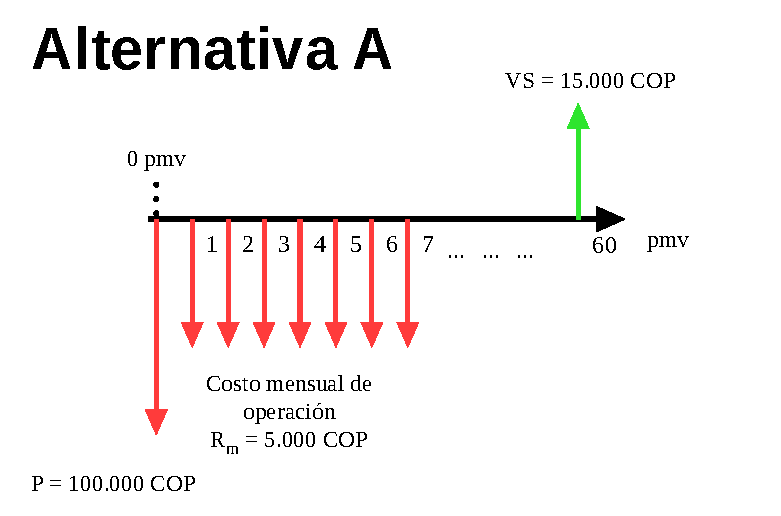
\includegraphics[trim=-5 -5 -5 -5, width=12cm, keepaspectratio]{10_Capitulo/img/ejemplos/PDFs/1/Ejemplo_1_A.pdf}}\\ \hline
		\multicolumn{3}{|c|}{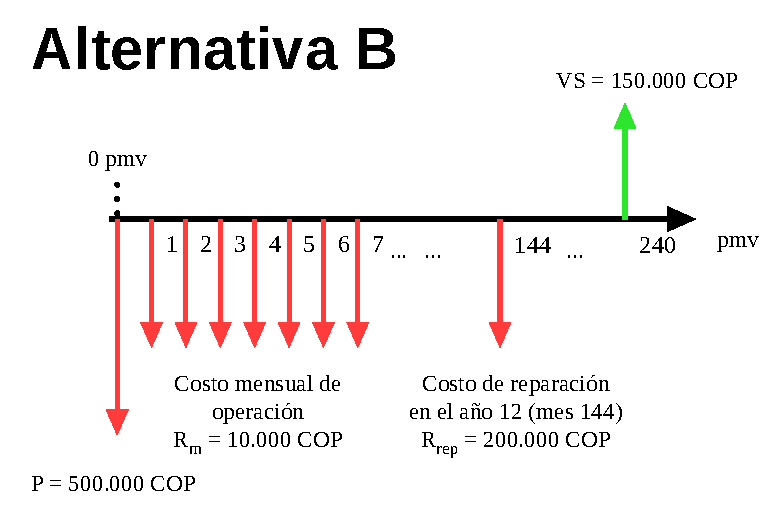
\includegraphics[trim=-5 -5 -5 -5, width=12cm, keepaspectratio]{10_Capitulo/img/ejemplos/PDFs/1/Ejemplo_1_B.pdf}}\\ \hline
		\multicolumn{3}{|p{14cm}|}{\small Los costos mensuales de operación se agrupan y acumulan al final de cada año; por eso el diagrama anual utiliza $i_{\text{año}}$ y períodos pav. La reparación de B ocurre al final del año 12.} \\ \hline

		%%%%% INICIO DECLARACIÓN FORMULAS
		\rowcolor[HTML]{FFB183}
		\multicolumn{3}{|c|}{\cellcolor[HTML]{FFB183}\textbf{4. Declaración de fórmulas}} \\ \hline

		\multicolumn{3}{|c|}{$i_m = \dfrac{j}{12} \quad ; \quad i_{\text{año}} = (1+i_m)^{12} - 1$}\\ 
		\multicolumn{3}{|c|}{$F_{op,\text{año}} = R_m \left[ \dfrac{(1+i_m)^{12}-1}{i_m} \right] \quad (F/A)$}\\
		\multicolumn{3}{|c|}{$A_P = P \left[ \dfrac{i(1+i)^n}{(1+i)^n-1} \right] \quad (A/P) \quad ; \quad A_F = F \left[ \dfrac{i}{(1+i)^n-1} \right] \quad (A/F)$}\\
		\multicolumn{3}{|c|}{$VP_{\text{rep}} = C_{\text{rep}}(1+i)^{-12} \quad ; \quad A_{\text{rep}} = VP_{\text{rep}} (A/P, i, 20)$}\\
		\multicolumn{3}{|c|}{$CAUE = \sum \text{Ingresos}_{\text{anualizados}} - \sum \text{Egresos}_{\text{anualizados}}$}\\
		\hline

		%%%%%% INICIO DESARROLLO MATEMÁTICO
		\rowcolor[HTML]{FFB183}
		\multicolumn{3}{|c|}{\cellcolor[HTML]{FFB183}\textbf{5. Desarrollo matemático}} \\ \hline

		\multicolumn{3}{|l|}{\textbf{Conversión de tasa:}} \\
		\multicolumn{3}{|l|}{$i_m = \dfrac{0{,}025}{12} = 0{,}002083333 = 0{,}208333\%\text{ pmv}$} \\
		\multicolumn{3}{|l|}{$i_{\text{año}} = (1 + 0{,}002083333)^{12} - 1 = 0{,}025288457 = 2{,}528846\%\text{ pav}$} \\ \hline

		\multicolumn{3}{|l|}{\textbf{Valor anual acumulado de los costos mensuales de operación:}} \\
		\multicolumn{3}{|l|}{Alternativa A: $F_{op,A} = 5.000 \cdot \dfrac{(1 + 0{,}002083333)^{12} - 1}{0{,}002083333} = \text{COP } 60.692{,}30/\text{año}$} \\
		\multicolumn{3}{|l|}{Alternativa B: $F_{op,B} = 10.000 \cdot \dfrac{(1 + 0{,}002083333)^{12} - 1}{0{,}002083333} = \text{COP } 121.384{,}59/\text{año}$} \\ \hline

		\cellcolor[HTML]{FFB183}\textbf{Componente anual equivalente} & \cellcolor[HTML]{FFB183}\textbf{Alternativa A (COP/año)} & \cellcolor[HTML]{FFB183}\textbf{Alternativa B (COP/año)} \\ \hline
		Recuperación de inversión inicial & $100.000(A/P, 2{,}528846\%, 5) = 21.542{,}56$ & $500.000(A/P, 2{,}528846\%, 20) = 32.161{,}02$ \\ \hline
		Costo mensual acumulado al cierre & $60.692{,}30$ & $121.384{,}59$ \\ \hline
		Reparación del año 12 & --- & $200.000(1{,}025288457)^{-12}(A/P, 2{,}528846\%, 20) = 9.533{,}16$ \\ \hline
		Crédito por salvamento & $15.000(A/F, 2{,}528846\%, 5) = 2.852{,}06$ & $150.000(A/F, 2{,}528846\%, 20) = 5.855{,}04$ \\ \hline

		\multicolumn{3}{|l|}{\textbf{CAUE de cada alternativa:}} \\
		\multicolumn{3}{|l|}{$CAUE_A = +2.852{,}06 - 21.542{,}56 - 60.692{,}30 = -\text{COP } 79.382{,}80/\text{año}$} \\
		\multicolumn{3}{|l|}{$CAUE_B = +5.855{,}04 - 32.161{,}02 - 9.533{,}16 - 121.384{,}59 = -\text{COP } 157.223{,}74/\text{año}$} \\ \hline

		%%%%%% INICIO RESPUESTA
		\rowcolor[HTML]{FFB183}
		\multicolumn{3}{|c|}{\cellcolor[HTML]{FFB183}\textbf{6. Respuesta}} \\ \hline

		\multicolumn{3}{|c|}{\parbox{14cm}{\centering\strut Se selecciona la alternativa A. Su CAUE es menos negativo y representa un costo anual equivalente menor: COP 79.382,80/año, frente a COP 157.223,74/año de la alternativa B.\strut}} \\ \hline
	\end{longtable}
\end{center}
%%%%%%%%%%%%%%%%%%%%%%%%%%FIN EJERCICIO 1 %%%%%%%%%%%%%%%%%%%%%%%%%%%


%%%%%%%%%% NO OLVIDAR COLOCAR ESTE COMENTARIO CON EL NUMERO DE EJERCICIO %%%%%%%%%%%%%
%%%%%%%%%%%%%%%%%%% EJERCICIO 2 %%%%%%
%%Text bf para negrilla , el \\ es para el salto de linea.
%%El primer \\ hace un espacio en el texto y el 2 \\ crea otro espacio
\textbf{Ejemplo 2}\newline
El jefe de producción de una fábrica debe decidir entre dos máquinas A y B. Las características de cada una son: \\
\begin{center}
		\begin{tabular}{|c|c|c|c|c|}
			\hline
			\rowcolor[HTML]{FFB183}
			\textbf{Maq.} & \textbf{P} & \textbf{n} & \textbf{VS} & \textbf{$R_a$} \\ \hline
			A            & 800.000 COP   & 3 años     & 200.000 COP    & 25.000 COP       \\ \hline
			B            & 600.000 COP   & 2 años     & 150.000 COP    & 30.000 COP       \\ \hline
		\end{tabular}
\end{center}

Con una tasa del 36\% nominal anual año vencido, determinar la mejor alternativa.

\textbf{Solución.}\\
\begin{center}
	\renewcommand{\arraystretch}{1.5}% Margenes de las celdas
	\small% Tamaño de letra de la tabla para que quepan las expresiones con COP
	%Creación de la cuadricula
	\begin{longtable}[H]{|c|c|c|}
		%Creamos una linea horizontal
		\hline
		%Definimos el color de la primera fila
		\rowcolor[HTML]{FFB183}
		%%%%% INICIO ASIGNACIÓN FECHA FOCAL %%%%%%%
		%%%%%%%%%% INICIO TITULO
		%Lo que se hace aquí es mezclar las 3 columnas en una sola
		\multicolumn{3}{|c|}{\cellcolor[HTML]{FFB183}\textbf{1. Asignación período focal}}   \\ \hline
		%%%%%%%%%% FIN TITULO
		%%%%% INICIO DECLARACIÓN DE VARIABLES %%%%%%%
		\multicolumn{3}{|c|}{$pf : 0  \textit{ pav }$} \\ \hline
		%Definimos el color de la primera fila
		\rowcolor[HTML]{FFB183}
		%%%%% INICIO DECLARACIÓN DE VARIABLES %%%%%%%
		%%%%%%%%%% INICIO TITULO
		\multicolumn{3}{|c|}{\cellcolor[HTML]{FFB183}\textbf{2. Declaración de variables}}                                                                                   \\ \hline
		%%%%%%%%%% FIN TITULO
		%%%%%%%%%% INICIO SUBTITULO
		\cellcolor[HTML]{FFB183}\textbf{Valores monetarios}    & 
		\cellcolor[HTML]{FFB183}\textbf{Valores no monetarios} &
		\cellcolor[HTML]{FFB183}\textbf{Incógnitas}  \\ \hline
		%%%%%%%%%% FIN SUBTITULO
		%%%%%%%%%% INICIO DE MATEMÁTICAS
		{Alternativa A} & \multicolumn{1}{|c|}{Alternativa A} & \multicolumn{1}{|c|}{Alternativa A}\\
    $P = 800{.}000\text{ COP}$ & $n_A =  3 \textit{ pav }$ & $CAUE_A =  \text{? COP}$\\
    $VS =  200{.}000\text{ COP}$ & $i_a= 36\% \textit{ pav }$ & \\
    $R_a = 25{.}000\text{ COP}$ & &\\
    {Alternativa B} & \multicolumn{1}{|c|}{Alternativa B} & \multicolumn{1}{|c|}{Alternativa B}\\
    $P = 600{.}000\text{ COP}$ & $n_B =  2 \textit{ pav }$& $CAUE_B =  \text{? COP}$\\
    $VS =  150{.}000\text{ COP}$& $i_b= 36\% \textit{ pav }$ & \\
    $R_b = 30{.}000\text{ COP}$& & \\\hline
		%%%%%%%%%% FIN DE MATEMÁTICAS
		%%%%% FIN DECLARACIÓN DE VARIABLES


		%%%%% INICIO FLUJO DE CAJA
		\rowcolor[HTML]{FFB183}
		\multicolumn{3}{|c|}{\cellcolor[HTML]{FFB183}\textbf{3. Diagrama de flujo de caja}}\\ 
        \hline
		%Mezclamos 3 columnas y pondremos el dibujo
		%%%%%%%%%%%%% INSERCIÓN DE LA IMAGEN
		
		\multicolumn{3}{|c|}{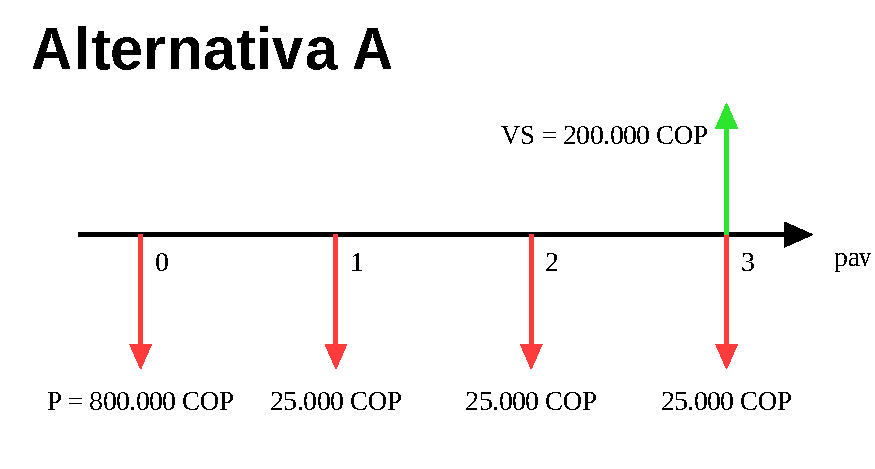
\includegraphics[trim=-5 -5 -5 -5, width=10.5cm, keepaspectratio]{10_Capitulo/img/ejemplos/PDFs/2/Ejemplo_2_A.pdf}}\\ \hline
		\multicolumn{3}{|c|}{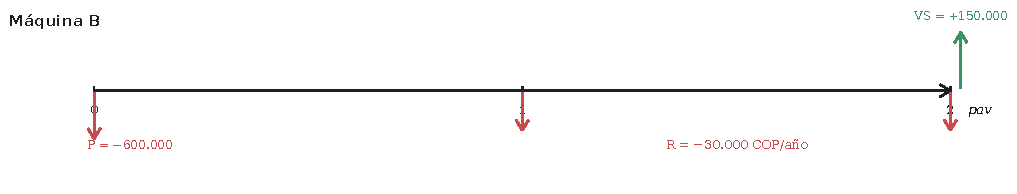
\includegraphics[trim=-5 -5 -5 -5, width=10.5cm, keepaspectratio]{10_Capitulo/img/ejemplos/PDFs/2/Ejemplo_2_B.pdf}}\\ \hline
		%%%%%%%%%%%%% FIN INSERCIÓN DE IMAGEN
		%%%%%FIN FLUJO DE CAJA

		%%%%% INICIO DECLARACIÓN FORMULAS
		%%%%%%%%%%% INICIO TITULO
		\rowcolor[HTML]{FFB183}
		\multicolumn{3}{|c|}{\cellcolor[HTML]{FFB183}\textbf{4. Declaración de fórmulas}} \\ \hline
		%%%%%%%%%%% FIN TITULO
  
		%%%%%%%%%%% INICIO MATEMÁTICAS
		\multicolumn{3}{|c|}{$VP=R\frac{1-(1+i)^{-n}}{i} \text{ Valor presente serie uniforme vencida}$}\\ 
		\multicolumn{3}{|c|}{$VF=R\frac{(1+i)^{n}-1}{i} \text{ Valor futuro serie uniforme vencida}$}\\
		\multicolumn{3}{|c|}{$CAUE = \sum \text{Ingresos}_{\text{anualizados}} - \sum \text{Egresos}_{\text{anualizados}} \text{ CAUE como sumatoria}$}\\
		\multicolumn{3}{|c|}{$A=P\frac{i}{1-(1+i)^{-n}} \text{ Recuperación de capital (serie uniforme vencida)}$}\\
		\multicolumn{3}{|c|}{$A=F\frac{i}{(1+i)^{n}-1} \text{ Fondo de amortización (serie uniforme vencida)}$}\\
		\hline
		%%%%%%%%%% FIN MATEMÁTICAS
  
		%%%%%% INICIO DESARROLLO MATEMÁTICO
		\rowcolor[HTML]{FFB183}
		%%%%%%%%%%INICIO TITULO
		\multicolumn{3}{|c|}{\cellcolor[HTML]{FFB183}\textbf{5. Desarrollo matemático}}   \\ \hline
		%%%%%%%%%% FIN TITULO
		%%%%%%%%%% INICIO MATEMÁTICAS
  
		Alternativa A & \multicolumn{2}{c|}{Alternativa B}\\ \hline

		\begin{tabular}[c]{@{}c@{}}Dividir los 800.000 COP \\ en 3 pagos anuales uniformes:\end{tabular} & \multicolumn{2}{c|}{\begin{tabular}[c]{@{}c@{}}Dividir los 600.000 COP \\ en 2 pagos anuales uniformes:\end{tabular}} \\
		$\begin{gathered}R_1 = 800{.}000\text{ COP}\mathbin{\color{red}\ast}\frac{0{,}36}{1-(1+0{,}36)^{-3}} \\ = 478{.}041{,}809\text{ COP}\end{gathered}$ & \multicolumn{2}{c|}{$\begin{gathered}R_1 = 600{.}000\text{ COP}\mathbin{\color{red}\ast}\frac{0{,}36}{1-(1+0{,}36)^{-2}} \\ = 470{.}237{,}288\text{ COP}\end{gathered}$}\\

        $ $  & \multicolumn{2}{c|}{}\\

        \begin{tabular}[c]{@{}c@{}}Dividir los 200.000 COP \\ en 3 pagos anuales uniformes:\end{tabular} & \multicolumn{2}{c|}{\begin{tabular}[c]{@{}c@{}}Dividir los 150.000 COP \\ en 2 pagos anuales uniformes:\end{tabular}} \\
		$\begin{gathered}R_2 = 200{.}000\text{ COP}\mathbin{\color{red}\ast}\frac{0{,}36}{(1+0{,}36)^{3}-1} \\ = 47{.}510{,}452\text{ COP}\end{gathered}$ & \multicolumn{2}{c|}{$\begin{gathered}R_2 = 150{.}000\text{ COP}\mathbin{\color{red}\ast}\frac{0{,}36}{(1+0{,}36)^{2}-1} \\ = 63{.}559{,}322\text{ COP}\end{gathered}$}\\

        $ $  & \multicolumn{2}{c|}{}\\

        $\begin{gathered}CAUE_{A} = -478{.}041{,}809\text{ COP} \\ - 25{.}000\text{ COP} + 47{.}510{,}452\text{ COP}\end{gathered}$ & \multicolumn{2}{c|}{$\begin{gathered}CAUE_{B} = -470{.}237{,}288\text{ COP} \\ - 30{.}000\text{ COP} + 63{.}559{,}322\text{ COP}\end{gathered}$}\\

        $ $  & \multicolumn{2}{c|}{}\\

        $CAUE_{A} = -455{.}531{,}357\text{ COP}$ & \multicolumn{2}{c|}{$CAUE_{B} = -436{.}677{,}966\text{ COP}$}\\

		\hline
		%%%%%%%%%% FIN MATEMÁTICAS
		%%%%%% FIN DESARROLLO MATEMÁTICO

		\rowcolor[HTML]{FFB183}
		\multicolumn{3}{|c|}{\cellcolor[HTML]{FFB183}\textbf{6. Respuesta}}    \\ \hline

		\multicolumn{3}{|c|}{La alternativa que representa menores pérdidas es la B.} \\ 
		\hline
	\end{longtable}
	%Se crean dos lineas en blanco para que no quede el siguiente texto tan pegado
	%\newline \newline
\end{center}
%%%%%%%%%%%%%%%%%%%%%%%%%%FIN EJERCICIO X %%%%%%%%%%%%%%%%%%%%%%%%%%%

%%%%%%%%%%% NO OLVIDAR COLOCAR ESTE COMENTARIO CON EL NUMERO DE EJERCICIO %%%%%%%%%%%%%
%%%%%%%%%%%%%%%%%%% EJERCICIO 3 %%%%%%
\textbf{Ejemplo 3. Selección entre dos proyectos de puente}\newline
Se presentan dos proyectos de puente. La alternativa A es un puente colgante con costo inicial de COP 850.000.000; el mantenimiento de la plataforma de asfalto cuesta COP 3.000.000 el primer año y aumenta COP 2.000.000 cada año. Cada cinco años se cambian los cables a un costo de COP 100.000.000. La alternativa B es un puente de concreto con costo inicial de COP 900.000.000; cada tres años se reacondicionan las bases por COP 25.000.000 y el mantenimiento anual es fijo de COP 5.000.000. Use una tasa del 24\% periódica anual vencida (pav).\\

\textbf{Solución.}\\

\begin{center}
	\renewcommand{\arraystretch}{1.5}% Margenes de las celdas
	\small% Tamaño de letra de la tabla para que quepan las expresiones con COP
	\begin{longtable}[H]{|c|c|c|}
		\hline
		\rowcolor[HTML]{FFB183}
		%%%%% INICIO ASIGNACIÓN FECHA FOCAL %%%%%%%
		\multicolumn{3}{|c|}{\cellcolor[HTML]{FFB183}\textbf{1. Asignación período focal}} \\ \hline
		\multicolumn{3}{|c|}{$pf = 0\text{ pav}$} \\ \hline
		
		%%%%% INICIO DECLARACIÓN DE VARIABLES %%%%%%%
		\rowcolor[HTML]{FFB183}
		\multicolumn{3}{|c|}{\cellcolor[HTML]{FFB183}\textbf{2. Declaración de variables}} \\ \hline
		\multicolumn{1}{|c|}{\cellcolor[HTML]{FFB183}\textbf{Valores monetarios}} &
		\multicolumn{1}{c|}{\cellcolor[HTML]{FFB183}\textbf{Valores no monetarios}} &
		\multicolumn{1}{c|}{\cellcolor[HTML]{FFB183}\textbf{Incógnitas}} \\ \hline
		
		$P_A = \text{COP } 850.000.000$ & $i = 24\%\text{ pav}$ & $CAUE_A = \text{? COP/año}$ \\
		$R_{1,A} = \text{COP } 3.000.000$ & $n_A = 5\text{ pav}$ & $CAUE_B = \text{? COP/año}$ \\
		$L_A = \text{COP } 2.000.000$ & $n_B = 3\text{ pav}$ & \\
		$C_{\text{cables},A} = \text{COP } 100.000.000\text{ en } t = 5$ & & \\
		$P_B = \text{COP } 900.000.000$ & & \\
		$R_B = \text{COP } 5.000.000/\text{año}$ & & \\
		$C_{\text{reac},B} = \text{COP } 25.000.000\text{ en } t = 3$ & & \\ \hline

		%%%%% INICIO FLUJO DE CAJA
		\rowcolor[HTML]{FFB183}
		\multicolumn{3}{|c|}{\cellcolor[HTML]{FFB183}\textbf{3. Diagrama de flujo de caja}} \\ \hline
		
		\multicolumn{3}{|c|}{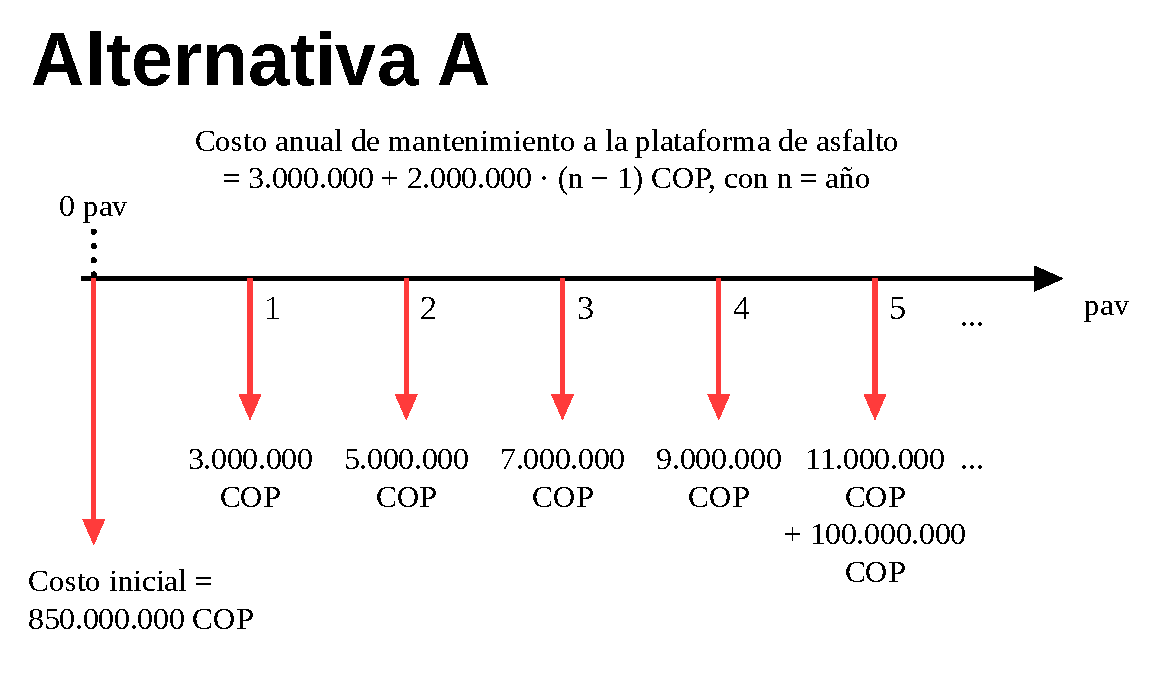
\includegraphics[trim=-5 -5 -5 -5, width=12cm, keepaspectratio]{10_Capitulo/img/ejemplos/PDFs/3/Ejemplo_3_A.pdf}}\\ \hline
		\multicolumn{3}{|c|}{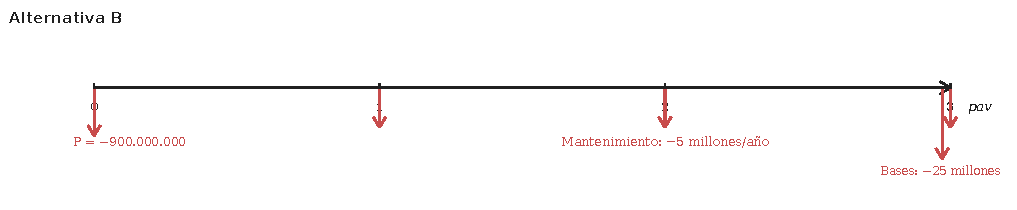
\includegraphics[trim=-5 -5 -5 -5, width=12cm, keepaspectratio]{10_Capitulo/img/ejemplos/PDFs/3/Ejemplo_3_B.pdf}}\\ \hline
		\multicolumn{3}{|p{14cm}|}{\small En A, el flujo de mantenimiento es un gradiente aritmético: $R_{t,A} = 3.000.000 + (t-1)(2.000.000)$, para $t = 1, 2, 3, 4, 5$. En B, el mantenimiento es uniforme y el reacondicionamiento ocurre al final del año 3.} \\ \hline

		%%%%% INICIO DECLARACIÓN FORMULAS
		\rowcolor[HTML]{FFB183}
		\multicolumn{3}{|c|}{\cellcolor[HTML]{FFB183}\textbf{4. Declaración de fórmulas}} \\ \hline

		\multicolumn{3}{|c|}{$CAUE = VPN \times (A/P, i, n)$}\\ 
		\multicolumn{3}{|c|}{$VPN = \sum F_t(1+i)^{-t} \quad \text{(cada egreso se registra con signo negativo)}$}\\
		\multicolumn{3}{|c|}{$A/P = \dfrac{i(1+i)^n}{(1+i)^n - 1} \quad ; \quad A/F = \dfrac{i}{(1+i)^n - 1}$}\\
		\hline

		%%%%%% INICIO DESARROLLO MATEMÁTICO
		\rowcolor[HTML]{FFB183}
		\multicolumn{3}{|c|}{\cellcolor[HTML]{FFB183}\textbf{5. Desarrollo matemático}} \\ \hline

		\multicolumn{3}{|l|}{\textbf{Alternativa A: puente colgante}} \\
		\multicolumn{3}{|p{14cm}|}{Primero se calcula el valor presente del gradiente de mantenimiento:} \\
		\multicolumn{3}{|p{14cm}|}{$VP_{\text{mant},A} = \dfrac{3.000.000}{1{,}24} + \dfrac{5.000.000}{1{,}24^2} + \dfrac{7.000.000}{1{,}24^3} + \dfrac{9.000.000}{1{,}24^4} + \dfrac{11.000.000}{1{,}24^5} = \text{COP } 16.901.534{,}21$.} \\
		\multicolumn{3}{|p{14cm}|}{$CAUE_A = -850.000.000(A/P, 24\%, 5) - VP_{\text{mant},A}(A/P, 24\%, 5) - 100.000.000(A/F, 24\%, 5)$} \\
		\multicolumn{3}{|p{14cm}|}{$CAUE_A = -309.610.557{,}64 - 6.156.345{,}21 - 12.424.771{,}49 = -\text{COP } 328.191.674{,}35/\text{año}$.} \\ \hline

		\multicolumn{3}{|l|}{\textbf{Alternativa B: puente de concreto}} \\
		\multicolumn{3}{|p{14cm}|}{$CAUE_B = -900.000.000(A/P, 24\%, 3) - 5.000.000 - 25.000.000(A/F, 24\%, 3)$} \\
		\multicolumn{3}{|p{14cm}|}{$CAUE_B = -454.246.505{,}72 - 5.000.000 - 6.617.958{,}49 = -\text{COP } 465.864.464{,}21/\text{año}$.} \\ \hline

		\rowcolor[HTML]{FFB183}
		\multicolumn{3}{|c|}{\textbf{Comparación}} \\ \hline
		\cellcolor[HTML]{FFB183} & \cellcolor[HTML]{FFB183}\textbf{A (COP/año)} & \cellcolor[HTML]{FFB183}\textbf{B (COP/año)} \\ \hline
		CAUE & $-328.191.674{,}35$ & $-465.864.464{,}21$ \\ \hline

		%%%%%% INICIO RESPUESTA
		\rowcolor[HTML]{FFB183}
		\multicolumn{3}{|c|}{\cellcolor[HTML]{FFB183}\textbf{6. Respuesta}} \\ \hline

		\multicolumn{3}{|c|}{\parbox{14cm}{\centering\strut Se selecciona la alternativa A. Su costo anual uniforme equivalente es menor: COP 328.191.674,35/año frente a COP 465.864.464,21/año de la alternativa B. La ventaja anual equivalente de A es COP 137.672.789,86.\strut}} \\ \hline
	\end{longtable}
\end{center}

\begin{center}
	\renewcommand{\arraystretch}{1.3}
	\begin{tabular}{|p{14.5cm}|}
		\hline
		\rowcolor[HTML]{FFB183}
		\textbf{Corrección sustancial del ejemplo 3} \\ \hline
		El cálculo original no anualizaba los costos iniciales de COP 850.000.000 y COP 900.000.000, y sumaba directamente costos anuales de mantenimiento. Además, la variable ``$VS$'' se utilizaba para un costo anual, aunque $VS$ corresponde a valor de salvamento. La solución corregida incluye las inversiones iniciales, descuenta los flujos extraordinarios y compara todos los costos en COP/año. \\ \hline
	\end{tabular}
\end{center}

\begin{center}
	\renewcommand{\arraystretch}{1.3}
	\begin{tabular}{|p{14.5cm}|}
		\hline
		\rowcolor[HTML]{FFB183}
		\textbf{Conclusión del capítulo} \\ \hline
		Antes de aplicar el CAUE, verificar que $i$ y $n$ tengan la misma periodicidad y modalidad; identificar la fecha de cada flujo; usar $A/P$ para anualizar un valor presente y $A/F$ para anualizar un valor futuro; y comparar las alternativas con el mismo convenio de signos. \\ \hline
	\end{tabular}
\end{center}
%%%%%%%%%%%%%%%%%%%%%%%%%%FIN EJERCICIO 3 %%%%%%%%%%%%%%%%%%%%%%%%%%%

